\documentclass[11pt]{article}
\usepackage[letterpaper,margin=0.72in]{geometry}
\usepackage{amsmath,amssymb,amsthm,mathtools}
\usepackage{graphicx,array,booktabs}
\usepackage[T1]{fontenc}
\usepackage{microtype}
\setlength{\parindent}{0pt}
\setlength{\parskip}{0.38em}
\setlength{\emergencystretch}{2em}
\newtheorem{theorem}{Theorem}
\newcommand{\R}{\mathbb R}
\newcommand{\Z}{\mathbb Z}
\newcommand{\card}[1]{\lvert#1\rvert}
\newcommand{\vol}[1]{\lvert#1\rvert}
\newcommand{\D}{\mathop\Delta}
\title{A finite-cell counterexample to higher-order Minkowski increments\\
\large A negative answer to Question 3.10 of arXiv:2206.01565}
\author{Run \texttt{fa\_banach\_001} --- \texttt{agent\_lane\_03}}
\date{12 August 2026}

\begin{document}
\maketitle

\textbf{Status.} High-confidence candidate full counterexample, pending
human review.  Question 3.10 is false at order $m=5$ in every dimension
$n\ge2$.

\section*{The source question}
For compact $A,B\subset\R^n$ with $0\in B$, put
$\D_B(A)=(A+B)\setminus A$.  The source proves its proposed inequality for
$m=2$ and asks whether, for every $m$, every compact $B_0$, and compact
$B_1,\ldots,B_m$ containing zero,
\begin{equation}\label{Q}
 \vol{\D_{B_1}\cdots\D_{B_m}(B_0)}\ge
 \sum_{S\subseteq[m]}(-1)^{m-|S|}
 \vol{B_0+\sum_{i\in S}B_i}.                             \tag{Q}
\end{equation}

\begin{center}
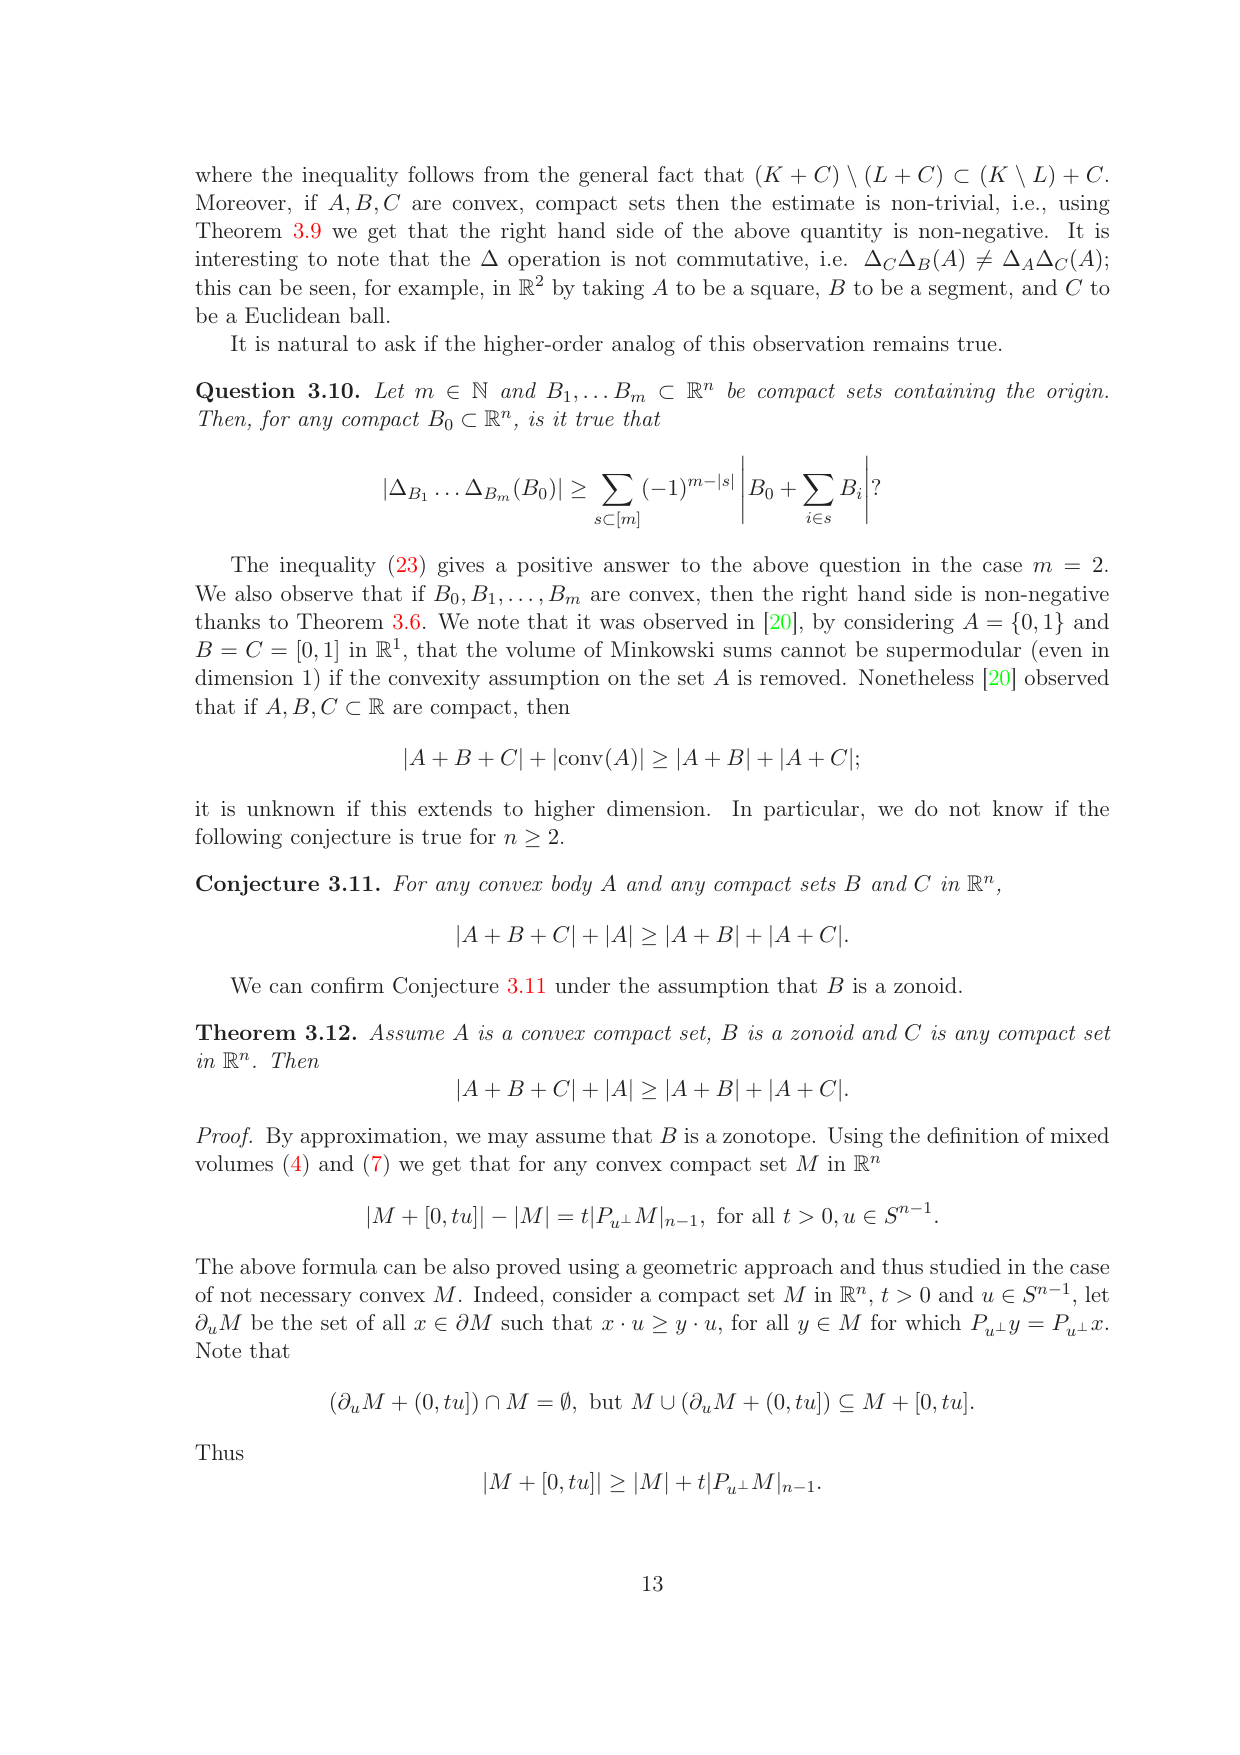
\includegraphics[width=0.75\textwidth,trim=35 390 35 135,clip]
 {figures/source_question_3_10_page_13.png}
\end{center}
The exact page is bundled as
\texttt{source\_excerpt\_question\_3\_10\_page\_13.pdf}.

\begin{theorem}\label{thm:main}
For every $n\ge2$ and every $0<\varepsilon<1$, there are a compact $B_0$
and finite compact sets $B_1,\ldots,B_5\subset\R^n$, each containing zero,
for which the left side of \eqref{Q} is $4\varepsilon^n$ and the right side
is $6\varepsilon^n$.  Hence \eqref{Q} is false.
\end{theorem}

\clearpage
\section*{The discrete configuration}
Work first in $\Z^2$.  Define
\begin{align*}
 E_0&=\{(-1,0),(1,-2),(-1,-2)\},\\
 P_1&=\{(-2,0),(-2,-1),(0,0)\},&
 P_2&=\{(1,0),(0,0)\},\\
 P_3&=\{(1,-1),(0,0)\},&
 P_4&=\{(0,-1),(0,0)\},\\
 P_5&=\{(2,-1),(-1,-1),(0,0)\}.&&
\end{align*}
For finite lattice sets put $\delta_P(E)=(E+P)\setminus E$ and recursively
$E_i=\delta_{P_i}(E_{i-1})$.  Direct set arithmetic gives
\begin{center}
\small
\begin{tabular}{ccl}
\toprule
$i$ & $\card{E_i}$ & $E_i$\\
\midrule
0&3&$\{(-1,0),(1,-2),(-1,-2)\}$\\
1&5&$\{(-3,0),(-3,-1),(-3,-2),(-3,-3),(-1,-3)\}$\\
2&5&$\{(-2,0),(-2,-1),(-2,-2),(-2,-3),(0,-3)\}$\\
3&5&$\{(-1,-1),(-1,-2),(-1,-3),(-1,-4),(1,-4)\}$\\
4&2&$\{(-1,-5),(1,-5)\}$\\
5&4&$\{(-2,-6),(0,-6),(1,-6),(3,-6)\}$\\
\bottomrule
\end{tabular}
\end{center}
Thus the iterated discrete increment has cardinality four.

For a mask $M\in\{0,1\}^5$, let
$P_M=\sum_{i:M_i=1}P_i$.  In binary-mask order from $00000$ to $11111$,
the $32$ values of $\card{E_0+P_M}$ are
\begin{align*}
 &(3,8,6,16,6,16,12,26,6,12,12,24,12,24,18,33,\\[-0.2em]
 &\hspace{2.2em}9,22,17,34,16,35,26,45,16,30,26,43,27,44,35,55).
\end{align*}
Grouping by Hamming weight $r=|M|$ gives respectively
\[
 (N_0,N_1,N_2,N_3,N_4,N_5)=(3,35,151,270,200,55).
\]
Therefore the fifth alternating difference is
\begin{equation}\label{six}
 -N_0+N_1-N_2+N_3-N_4+N_5
 =-3+35-151+270-200+55=6.                              \tag{1}
\end{equation}

\section*{Exact lift to compact subsets of $\R^n$}
Embed every displayed lattice point in the first two coordinates of $\Z^n$
and let $Q=[0,\varepsilon]^n$.  For finite $E\subset\Z^2$ write
\[
 \Phi(E)=(E\times\{0\}^{n-2})+Q.
\]
Because $0<\varepsilon<1$, distinct cubes in $\Phi(E)$ have positive
separation.  Consequently, for all finite lattice sets $E,F,P$,
\begin{equation}\label{functor}
 \Phi(E)+P=\Phi(E+P),\qquad
 \Phi(E)\setminus\Phi(F)=\Phi(E\setminus F),\qquad
 \vol{\Phi(E)}=\card{E}\varepsilon^n,                   \tag{2}
\end{equation}
where $P$ is embedded in the same coordinate plane.  The middle equality is
used only for unions of cells from this common lattice family.

Take $B_0=\Phi(E_0)$ and take the five increment sets to be the finite
embedded sets $P_i$.  Every $P_i$ contains zero.  From \eqref{functor},
if $D_0=B_0$ and $D_i=\D_{P_i}(D_{i-1})$, then
$D_i=\Phi(E_i)$.  Hence
\[
 \vol{\D_{P_5}\D_{P_4}\D_{P_3}\D_{P_2}\D_{P_1}(B_0)}
 =\vol{D_5}=4\varepsilon^n.                              \tag{3}
\]
The right side of \eqref{Q} is symmetric in its five increment sets, and
\eqref{functor}--\eqref{six} show that it equals $6\varepsilon^n$.
Thus, taking the source labels $(B_1,\ldots,B_5)=(P_5,\ldots,P_1)$ if its
composition is read outermost first, \eqref{Q} asserts
$4\varepsilon^n\ge6\varepsilon^n$, a contradiction.  This proves Theorem
\ref{thm:main}. \qed

\section*{Proof intuition and scope}
Separated lattice cubes turn Minkowski addition by a finite lattice set into
ordinary finite sumset formation, while $\D$ becomes literal set difference
of cell indices.  The question therefore contains a purely finite
combinatorial assertion.  At the fifth iteration the boundary operation
collapses the configuration to four cells, but the fifth alternating sum of
all Minkowski expansions still counts six cells' worth of volume.

The construction disproves the universal question for $m=5$ and all
$n\ge2$.  It makes no claim about $m=3$ or $m=4$, about a convex $B_0$, or
about the paper's separate Conjecture 3.11.  Exact-title, exact-question, and
official-arXiv searches through 12 August 2026 found no later explicit answer;
this is a bounded novelty audit, not a priority claim.

\section*{Verification and reference}
The bundled \texttt{verifier.py} recomputes all six stages, all $32$ subset
cardinalities, the grouped totals, and the strict deficit using only exact
integer set arithmetic.

\textbf{[1]} M. Fradelizi, M. Madiman, and A. Zvavitch,
\emph{Sumset estimates in convex geometry}, arXiv:2206.01565,
Question 3.10, p.~13.

\end{document}
